\documentclass[12pt]{article}

\usepackage{amsmath,amssymb,amsthm,bm}
\usepackage[margin=1in]{geometry}
\usepackage{titling}
\usepackage{subcaption}
\usepackage{setspace}
\usepackage{graphicx}
\graphicspath{ {images/} }


\doublespacing
\theoremstyle{plain}
\newtheorem{theorem}{Theorem}[section]
\newtheorem{corollary}{Corollary}[theorem]
\newtheorem{lemma}[theorem]{Lemma}
\newtheorem{definition}{Definition}

\newcommand{\R}{\mathbb{R}}
\newcommand{\Z}{\mathbb{Z}}
\newcommand{\C}{\mathbb{C}}

\title{An Exploration of the Riemann Hypothesis}
\author{Lukas Zamora}
\date{MATH 220 -- 903\\Topic 27}

\begin{document}

	\begin{titlingpage}
		\maketitle
		\begin{abstract}
			The Riemann Hypothesis is a conjecture made in 1859 by Bernhard Riemann stating that all the complex zeros of the zeta function $ \zeta(s) $ lie on a `critical line' where the function's real part is equal to $ 1/2 $. To this day it has not been proven, despite numerous efforts by mathematicians. If solved, this hypothesis could have an immense impact on prime number distributions, which has applications in areas such as cybersecurity.
		\end{abstract}
	\end{titlingpage}

	\pagenumbering{roman}

	\tableofcontents

	\newpage

	\pagenumbering{arabic}
	
	\section{Introduction}

	On August 8, 1900, David Hilbert (Figure \ref{fig:hilbert}), a prominent German mathematician, presented a list of ten problems at the International Congress of Mathematicians in Paris that he felt would be of fundamental importance in the 20th century. After these problems were met with critical acclaim, Hilbert announced thirteen extra problems (twenty-three in total). These problems, much like their predecessors, were also met with great critical acclaim. Today, seventeen of the twenty-three problems have been completely solved or partially solved. Many of these questions resulted in breakthroughs in modern mathematics.
	
	One the problems from Hilbert's list, named the Riemann Hypothesis, is undoubtedly one of the most famous problems in 21st century mathematics. It was first posed by Bernhard Riemann (Figure \ref{fig:riemann}), famously known for the first rigorous definition of the integral of a function on an interval. In his paper titled ``Ueber die Anzahl der Primzahlen unter einer gegebenen Gr\"{o}sse" (translated to ``On the Number of Prime Numbers less than a Given Quantity"), Riemann presents the zeta function (first posed by Euler), analytic continuation of this function, and most importantly, the Riemann Hypothesis. We will explore these topics further, and discuss their significance for important areas in mathematics.
	
	\section{The Zeta Function}

	To understand the Riemann Hypothesis, one must first introduce the zeta function, since it is the backbone to this hypothesis. Suppose we are given the following infinite sum, 
	\[ 1 + \frac{1}{2} + \frac{1}{3} + \frac{1}{4} + \frac{1}{5} + \ldots \]
	and would like to know if it converges or diverges, i.e. approach some finite number, or trail off to infinity. In this case, this sum diverges. This does not really tell us much, so let us try a different sum:
	\[ 1 + \frac{1}{2^2} + \frac{1}{3^2} + \frac{1}{4^2} + \frac{1}{5^2} + \ldots \]
	This problem is a little more special. In 1735, at the age of 24, Leonard Euler (Figure \ref{fig:euler}) proved that this sum converges to $ \dfrac{\pi^2}{6} $ \cite{zeta(2)}. This problem is known as the Basel Problem. Euler started his derivation with the Taylor series of $ \sin(x) $,
	\[ \sin(x) = x - \frac{x^3}{3!} + \frac{x^5}{5!} - \frac{x^7}{7!} + \dots \]
	Dividing through by $ x $, we have
	\begin{equation}\label{sin}
		\frac{\sin(x)}{x} = 1 - \frac{x^2}{3!} + \frac{x^4}{5!} - \frac{x^6}{7!} + \dots
	\end{equation}
	Notice that $ \sin(x) = 0 $ at $ 0, \, \pi, \, 2\pi, \, 3\pi $, etc. Euler used what is known as the Weierstrass factorization theorem, which states that functions can be represented by a product involving their zeros, to show that the left hand side of (\ref{sin}) can be written as a product of linear factors given by its roots:
	\begin{align*}
		\frac{\sin(x)}{x} &= \left( 1 - \frac{x}{\pi} \right) \left( 1 + \frac{x}{\pi} \right) \left( 1 - \frac{x}{2\pi} \right) \left( 1 + \frac{x}{2\pi} \right) \left( 1 - \frac{x}{3\pi} \right) \left( 1 + \frac{x}{3\pi} \right) \dots\\
		&= \left( 1 - \frac{x^2}{\pi^2} \right) \left( 1 - \frac{x^2}{4\pi^2} \right) \left( 1 - \frac{x^2}{9\pi^2} \right) \dots
	\end{align*}
	If we multiply out this product and collect all the $ x^2 $ terms, we see that the $ x^2 $ coefficient of $ \frac{\sin(x)}{x} $ is,
	\[ - \left( \frac{1}{\pi^2} + \frac{1}{4\pi^2} + \frac{1}{9\pi^2} + \cdots \right) = -\frac{1}{\pi^2} \sum\limits_{n=1}^{\infty} \frac{1}{n^2} \]
	But from the original infinite series expansion of $ \frac{\sin(x)}{x} $, the coefficient of $ x^2 $ is $ -\frac{1}{3!} = -\frac{1}{6} $. These coefficients must be equal; therefore,
	\[ 	-\frac{1}{6} = -\frac{1}{\pi^2} \sum\limits_{n=1}^{\infty} \frac{1}{n^2} \]
	or, 
	\[ \sum\limits_{n=1}^{\infty} \frac{1}{n^2} = \frac{\pi^2}{6} \]
	Euler went on to formulate a more general definition, 
	\begin{definition}
		For $ s \in \Z, s \geq 1 $,
			\[ Z(s) = \sum\limits_{n=1}^{\infty} \frac{1}{n^s} = \frac{1}{1^s} + \frac{1}{2^s} + \frac{1}{3^s} + \frac{1}{4^s} + \frac{1}{5^s} + \ldots \]
	\end{definition}
	Euler then wondered if there are any other places where $ Z(s) $ converges. In fact there are \textit{a lot} of places where $ Z(s) $ converges, and we will see that in a later section.
	
	In 1859, in his only paper on number theory, Bernhard Riemann, using analytic continuation, showed that,
	\[ \zeta(s) = \frac{1}{1 - 2^{1-s}} \sum\limits_{n=0}^{\infty} \frac{1}{2^n+1} \sum\limits_{k=0}^{\infty} (-1)^k \frac{n!}{k!(n-k)!}(k+1)^{-s}. \]
	While daunting at first, if we observe closely, we see that $ \zeta(2) = \dfrac{\pi^2}{6} $,the same exact value that Euler proved for $ Z(s) $. Riemann concluded that for values where $ Z(s) $ converges, $ Z(s) = \zeta(s) $ \cite{riemann}. This function $ \zeta(s) $ is known as the \textit{Riemann zeta function}. Riemann also extended this idea of $ s \in \Z $ to $ s \in \C $ by the use of analytic continuation (extending the domain of the function). This opens a lot more doors, since $ s $ is now defined as a complex number. However, $ \zeta(1) $ is still undefined.
	
	\subsection{Euler's Relationship with $ \zeta(s) $}
	
	In the 18th century, Euler found an analytic proof of the infinitude of the primes by making use of a factorization formula he had discovered for the Riemann zeta function. Starting with the definition of $ \zeta(s) $ he found that 
	\[ \left(1 - \frac{1}{2^s} \right ) \zeta(s) = 1 + \frac{1}{3^s} + \frac{1}{5^s} + \frac{1}{7^s} + \frac{1}{9^s} + \ldots \]
	which eliminated all the even terms, that is, all terms that are divisible by 2. Then by multiplying this expression by $ \dfrac{1}{3^s} $ and subtracting the result, he found that he canceled out the terms that were multiples of 3 that were not canceled out in the first step. Thus
	\begin{align*}
		\left(1 - \frac{1}{2^s} \right) \zeta(s) &= 1 + \frac{1}{3^s} + \frac{1}{5^s} + \frac{1}{7^s} + \frac{1}{9^s} + \ldots\\
		\left(1 - \frac{1}{3^s} \right) \left(1 - \frac{1}{2^s} \right) \zeta(s) &= 1 + \frac{1}{5^s} + \frac{1}{7^s} + \frac{1}{11^s} + \frac{1}{13^s} + \frac{1}{17^s} + \ldots
	\end{align*}
	Then if you continue in this way, in each step multiplying by a prime number the expressions and then subtracting, all terms start to cancel out, and in the limit what will be left on the right hand side is just 1, and on the left hand side we will have a product over each prime number multiplying the zeta function as follows
	\[ \zeta(s) \left(1 - \frac{1}{2^s} \right) \left(1 - \frac{1}{3^s} \right) \left(1 - \frac{1}{5^s} \right) \left(1 - \frac{1}{7^s} \right) \ldots = 1. \]
	From this we obtain the factorization of the zeta function discovered by Euler
	\[ \zeta(s) = \frac{1}{\left(1 - \frac{1}{2^s} \right) \left(1 - \frac{1}{3^s} \right) \left(1 - \frac{1}{5^s} \right) \left(1 - \frac{1}{7^s} \right) \ldots}. \]
	Or how it is more commonly written, 
	\[ \zeta(s) = \prod_{\text{prime} \, p} \frac{1}{1-p^{-s}}, \]
	where the $ \Pi $ operator is the Euler product.
	
	
	\subsection{Non-trivial Zeros}
	
	Back in the 1700s when Euler studied $ \zeta(s) $, he found that $ \zeta(s) = 0 $ when $ s = -2k $ for some $ k \in \Z $. Although interesting, it does not really tell us much. These values of $ s $ are called \textit{trivial zeros}. Upon further investigation, Riemann found some more values of $ s $ where $ \zeta(s) = 0 $,
	\begin{align*}
		\zeta(\frac{1}{2} + 21.022039639 i) &= 0\\
		\zeta(\frac{1}{2} + 25.010857580 i) &= 0\\
		\zeta(\frac{1}{2} + 30.424876126 i) &= 0.
	\end{align*}
	These values are known as \textit{non-trivial zeros}. Riemann saw this pattern of $ s $ equaling to $ \dfrac{1}{2} $ plus some multiple of $ i $ for when $ \zeta(s) = 0 $, and came up with the following hypothesis,
	\subsection{Riemann's Hypothesis.} \textit{If} $ \zeta(s) = 0 $ \textit{and} $ s $ \textit{is not a negative even integer then} $ s = \dfrac{1}{2} + it $ \textit{for some} $ t \in \R $.\\
	
	\noindent This hypothesis is considered by many mathematicians to be the most important unsolved problem in mathematics today.
	
	
	\section{Applications of the Riemann Hypothesis}
	
	\subsection{The Prime Number Theorem}

	One of main reasons why the Riemann Hypothesis is so popular is that it is used to determine the distributivity of prime numbers in a certain interval. In 1792, Carl Friedrich Gauss (Figure \ref{fig:gauss}) was studying the number of primes up to a certain number. He concluded that the number of primes less than $ x $ is about $ \dfrac{x}{\ln(x)} $. We now define the following,
	\begin{definition}
		 The number of primes less than $ x $ is defined to be 
		 \[ \pi(x) \sim \frac{x}{\ln(x)} \]
		 Meaning $ \pi(x) $ is asymptotic to $ \dfrac{x}{\ln(x)} $ as $ x \to \infty $, as illustrated in Figure \ref{fig:pix}.
	\end{definition}
	 At the time this was a very reasonable estimate. Wanting to find a more accurate estimate, Gauss defined the following function,
	\begin{definition}
		The offset logarithmic integral function is defined to be
		\[ Li(x) = \int_2^x \frac{dt}{\ln(t)} \]
	\end{definition}
	And posed that $ \pi(x) \sim Li(x) $. Which was an improvement from his previous hypothesis. This brings us to the following theorem,
	\begin{theorem}[Prime Number Theorem]
		The number of primes less than $ x $ is approximately $ Li(x) $.
	\end{theorem}
	One may now ask, ``how far apart do $ Li(x) $ and $ \pi(x) $ get? The difference between $ Li(x) $ and $ \pi(x) $ is known as the \textit{error term in the Prime Number Theorem}. It has been shown that $ Li(x) $ and $ \pi(x) $ can differ by as much as $ \sqrt{x} \cdot \ln(x) $, which was proven by van Koch in 1901\cite{koch}. But if the Riemann Hypothesis was indeed to be true, then $ Li(x) $ and $ \pi(x) $ never differ by more than about $ \sqrt{x} \cdot \ln(x) $. Conversely, if $ Li(x) $ and $ \pi(x) $ never differ by more than about $ \sqrt{x} \cdot \ln(x) $, then the Riemann Hypothesis is true. 
	
	\subsection{The Critical Line}
	
	All of the non-trivial zeros that Riemann calculated lay on what is called the \textit{critical line} (Figure \ref{fig:critical_line}). He posed that these non-trivial zeros all must lie in a vertical strip one unit wide (the ``critical strip"), centered on the critical line. In the 1800s, it was shown that the Prime Number Theorem would be true if the non-trivial zeros could all be shown to lie properly \textit{inside} the critical strip, that is, not on its edges. In 1896, the mathematicians Hadamard and de la Vall\'{e}e Poussin proved this almost simultaneously, thereby proving the Prime Number Theorem.
	
	Further narrowing the strip in which the non-trivial zeros are all known to lie would lead to more precise information on the distribution of prime numbers. The ultimate achievement would be to reduce this strip to its central line, as narrow as it is possible to get. If this can be done, the Riemann Hypothesis is proved, and we would know that the prime numbers are as ``well behaved" as possible. If the Riemann Hypothesis is false, there will be non-trivial zeros which do not lie on the critical line, resulting in huge fluctuations in the distribution of primes.
	
	\subsection{RSA Cryptography}
	
	The RSA algorithm, most commonly used in cryptography, involves the use of \textit{very} large prime numbers and exploits the fact that determining the prime factors of a large composite number is much more strenuous than multiplying the factors together in the first place. If a proof of the Riemann Hypothesis was to emerge, it would not compromise the RSA algorithm itself. Rather, the idea(s) needed to prove the Riemann Hypothesis could potentially lead to breakthroughs in large integer factorization, which would be an enormous problem for RSA cryptography.
	
	
	\section{Conclusion}
	
	The Riemann Hypothesis is a cornerstone problem in number theory that, if proven, could unlock the secrets of prime number distributions. Having been unsolved for over 150 years, it continues to stumble the most prestigious of mathematicians. Since the death of Bernhard Riemann, his groundbreaking paper has stood a landmark in prime number theory. Numerous new results and conjectures associated with the hypothesis are published every year, in the hope that one day a proof will be solved.
	
	
	


	\newpage

	\begin{thebibliography}{9}
		\bibitem{zeta(2)} 
		Robin Chapman. \textit{``Evaluating $ \zeta(2) $."} Department of Mathematics University of Exeter, 1999.
		\verb|https://empslocal.ex.ac.uk/people/staff/rjchapma/etc/zeta2.pdf|
		
		\bibitem{riemann} 
		Bernhard Riemann. \textit{On the Number of Prime Numbers less than a Given Quantity.} 
		\textit{Ueber die Anzahl der Primzahlen unter
			einer gegebenen Gr\"{o}sse}. (German) 
		Monatsberichte der Berliner Akademie, November 1859.
		
		\bibitem{koch} 
		H. von Koch, \textit{Acta Mathematica}, 24 (1901), 159-182. 
	\end{thebibliography}
	\addcontentsline{toc}{section}{References}

	
	\newpage
	
	\section*{Appendix A: Figures}
	
	
	\begin{figure}[h!]
		\centering
		\begin{minipage}{.5\textwidth}
			\centering
			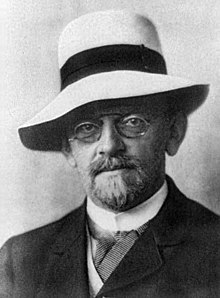
\includegraphics[width=.4\linewidth]{hilbert.jpg}
			\captionof{figure}{David Hilbert}
			\label{fig:hilbert}
		\end{minipage}%
		\begin{minipage}{.5\textwidth}
			\centering
			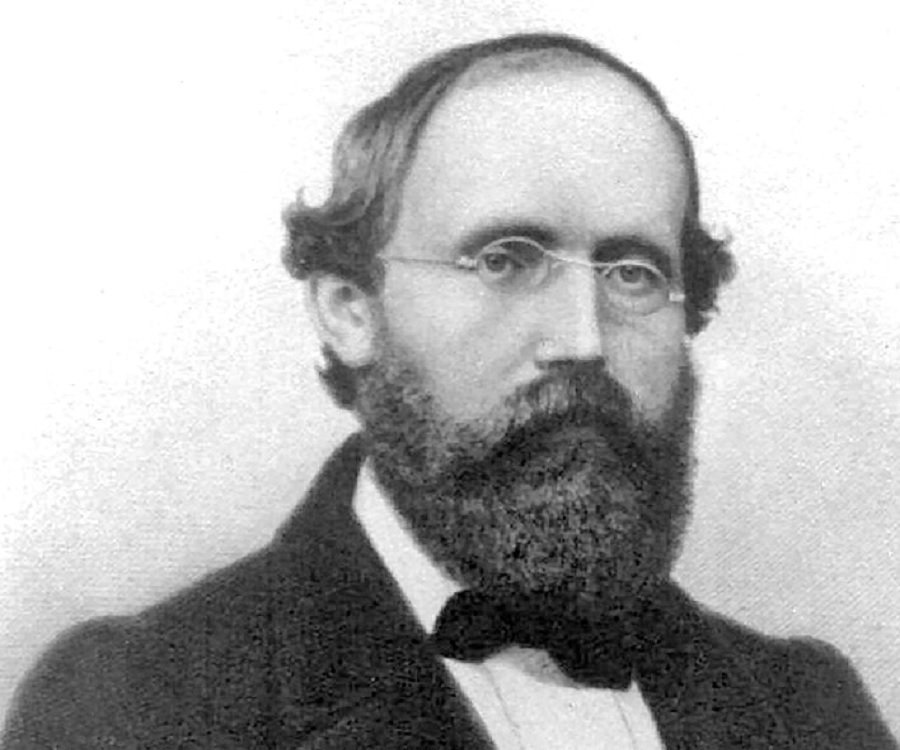
\includegraphics[width=.4\linewidth]{riemann.jpg}
			\captionof{figure}{Bernhard Riemann}
			\label{fig:riemann}
		\end{minipage}
	\end{figure}

	\begin{figure}[h!]
		\begin{minipage}{.5\textwidth}
			\centering
			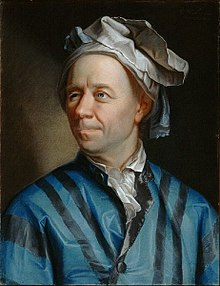
\includegraphics[width=.4\linewidth]{euler.jpg}
			\captionof{figure}{Leonard Euler}
			\label{fig:euler}
		\end{minipage}
		\begin{minipage}{.5\textwidth}
			\centering
			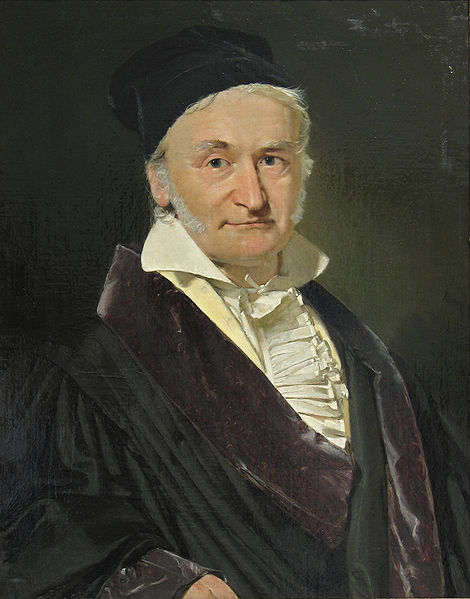
\includegraphics[width=.4\linewidth]{gauss.jpg}
			\captionof{figure}{Carl Friedrich Gauss}
			\label{fig:gauss}
		\end{minipage}
	\end{figure}


		\begin{figure}[t]
			\centering
			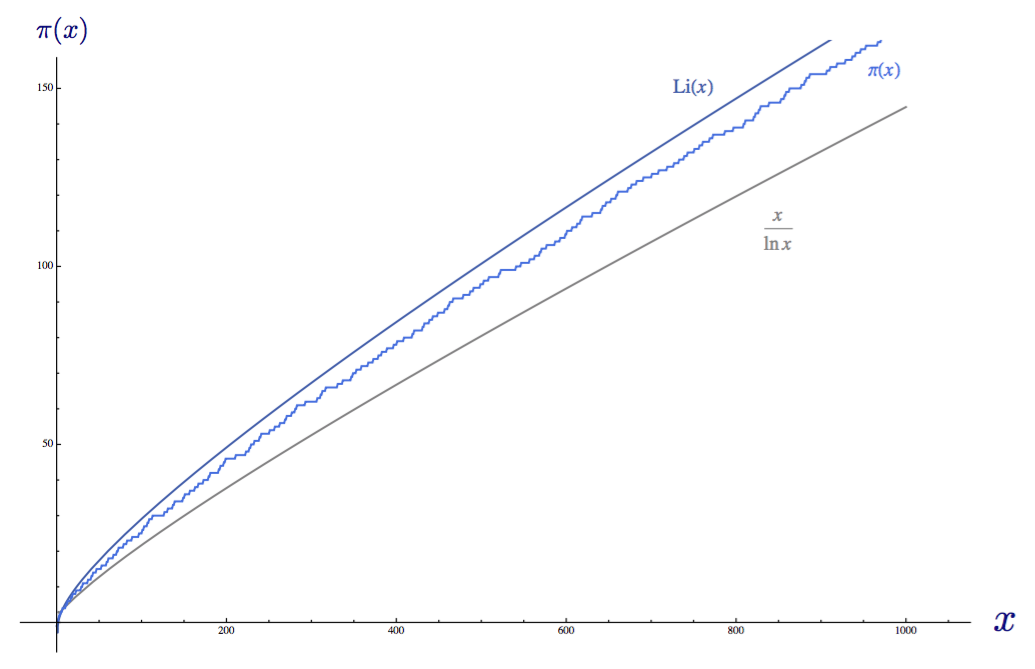
\includegraphics[scale=.4]{pix.png}
			\caption{Comparison of $ \pi(x) $ and other approximations}
			\label{fig:pix}
			
			\centering
			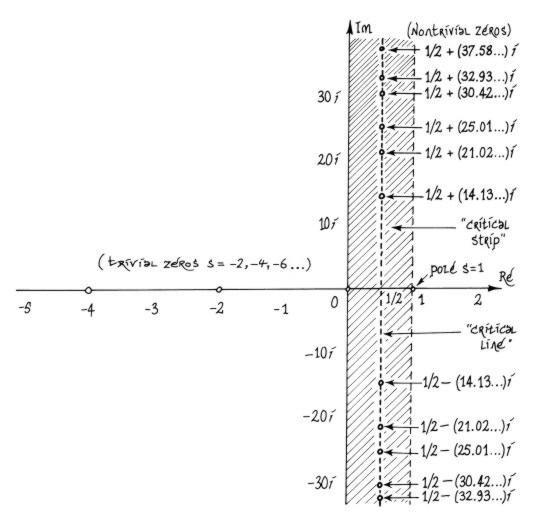
\includegraphics[scale=.5]{critical_line.jpg}
			\caption{The Critical Line}
			\label{fig:critical_line}
		\end{figure}		


	
	\addcontentsline{toc}{section}{Appendix A: Figures and Tables}


\end{document}
